% Chapter 1

\chapter{Introducción general} % Main chapter title

\label{Chapter1} % For referencing the chapter elsewhere, use \ref{Chapter1} 
\label{IntroGeneral}

%----------------------------------------------------------------------------------------

% Define some commands to keep the formatting separated from the content 
\newcommand{\keyword}[1]{\textbf{#1}}
\newcommand{\tabhead}[1]{\textbf{#1}}
\newcommand{\code}[1]{\texttt{#1}}
\newcommand{\file}[1]{\texttt{\bfseries#1}}
\newcommand{\option}[1]{\texttt{\itshape#1}}
\newcommand{\grados}{$^{\circ}$}

%----------------------------------------------------------------------------------------

%\section{Introducción}

%----------------------------------------------------------------------------------------
En este capítulo se expone la problemática, su contexto y el portafolio de opciones que se encuentran disponibles para darle solución. De igual manera, se hace una descripción rápida de cómo se acotó el problema a fin de poder generar un mínimo producto viable.

\section{Contexto de la problemática}

El uso de cámaras de vídeo es una práctica extremadamente común en el negocio de la seguridad. Su uso puede mejorar el área de cobertura de vigilancia \cite{5}, mientras que al mismo tiempo reduce la cantidad de personal empleado en hacer rondas de seguridad. Sin embargo, tener cámaras estáticas implica que será necesario contar con más de ellas \cite{4}, que a la vez tendrán que ser revisadas por varias personas.

La propuesta abordada en este trabajo busca solucionar estos dos problemas a través de la creación de un módulo de inteligencia artificial que permita el análisis automático de varios \textit{streamings} de vídeo provenientes de cámaras montadas en drones, y sea capaz de responder a estos estímulos digitales, al pasarle la información del intruso encontrado al software del que hará parte.

Esto permitirá que haya un análisis mucho más preciso y a menor costo de lo que era posible anteriormente, teniendo en cuenta que los drones podrán abarcar un área mucho mayor, y que no se dependerá de la concentración de una persona para encontrar intrusos. Esto implica que el sistema deberá estar en capacidad de analizar más de un \textit{streaming} de video al tiempo. Igualmente, el uso de estas tecnologías permite la utilización de cámaras infrarrojas, lo que hace posible la identificación de intrusos en la noche, cuando el ojo humano es incapaz de distinguir. 

Dado que este sistema hará parte de un módulo más grande, se decidió que, dentro de los requisitos, el sistema no deberá tomar decisiones basadas en sus hallazgos, sino simplemente comunicarlos tanto a otro sistema (del que hace parte), como al personal de seguridad encargado.


\section{Motivación}

Este trabajo responde a cinco necesidades concretas del ámbito de la vigilancia. Estas necesidades son:

\begin{itemize}
	\item Razones económicas: teniendo en cuenta que, al reducir al personal encargado de hacer seguimiento a las cámaras, o de hacer rondas de seguridad en horarios determinados, es posible reducir costos. De igual manera, el uso de drones permite una reducción sustancial en el número de cámaras que deberán ser instaladas, cosa que resulta particularmente útil en grandes áreas y permitirá una reducción muy importante en los costos de mantenimiento asociados. 
%	\item Calidad de la vigilancia: dado que el trabajo de gran parte del personal de vigilancia tiene la particularidad de que puede volverse muy monótono. Esto teniendo en cuenta que es un trabajo en el que se espera que no suceda nada. Sin embargo, es de vital importancia cuando esto deja de cumplirse, dado que hay algún evento que pueda afectar la seguridad.
	
Al ser tan monótono, es muy probable que el personal encargado se vea expuesto a distracciones, que pueden tener consecuencias severas en el momento en el que se presente algún evento que comprometa la seguridad. La situación se puede agravar en caso de tener una gran cantidad de cámaras, dado que el estar constantemente obligados a supervisarlas puede generar niveles no razonables de carga en el personal.

	\item Velocidad de reacción: una vez identificada una potencial amenaza, a través del sistema encargado de controlar los drones se podrá enviar órdenes a los equipos a fin de tomar mejores decisiones para manejar la situación. Es por esto que es de vital importancia que el módulo de inteligencia artificial encargado de la detección de los intrusos también sea capaz de hacerlo en tiempos razonables, que en este caso, han sido definidos por el cliente y se encuentran por debajo de los 4 segundos. Este valor se ha calculado a partir de la velocidad esperada de vuelo de los drones de hasta 30 km/h, lo que otorga un radio máximo de 33 metros entre detecciones.  Cabe anotar, sin embargo, que el tiempo ideal es menor o igual a un segundo, lo que genera un radio de 8 metros aproximadamente. 
	
	\item Aporte de pruebas: los drones (a través de la necesidad de velocidad de reacción) son un método ideal para aportar pruebas confiables de los hechos. Es así como un modelo de inteligencia artificial permite generar una mayor claridad en la interpretación de las pruebas aportadas, lo que puede generar una mejor comprensión y análisis de los hechos por parte de todos los implicados.
	
	\item Identificación de intrusos en horas de la noche: teniendo en cuenta que los modelos de inteligencia artficial pueden ser capaces de identificar las clases requeridas con diferentes condiciones de iluminación, puede ayudar a la identificación de intrusos cuando las condiciones de iluminación no son ideales. Por otro lado, es muy probable que esto sea mejorado sustancialmente con el uso de cámaras infrarrojas. 

\end{itemize}

Este tipo de propuestas, sin embargo, no se han hecho posibles hasta hace relativamente poco, cuando los modelos de inteligencia artificial alcanzaron una madurez que permite que no requieran grandes capacidades computacionales para poder ser ejecutados, de forma que implementarlos no requiera una inversión importante en equipos de cómputo.

\section{Estado del arte}

Existen varias técnicas y varios modelos que se pueden utilizar para implementar visión por computadora. Uno de los métodos más comunes a la fecha es el algoritmo YOLO, que se caracteriza por ser el primer modelo que no requiere hacer un doble análisis de la imagen \citep{1} (de aquí proviene su nombre: \textit{You Only Look Once}), y en consecuencia, analiza las imágenes en un tiempo mucho menor. 


% Please add the following required packages to your document preamble:
% \usepackage{booktabs}
\begin{table}[]
\centering
\caption{Fecha de lanzamiento de distintos modelos YOLO.}
\label{fechas-lanzamiento}
\begin{tabular}{@{}ll@{}}
\toprule
\multicolumn{1}{c}{\textbf{Versión}} & \multicolumn{1}{c}{\textbf{Fecha de lanzamiento}} \\ \midrule
YOLOv3                      & Abril de 2018                            \\
YOLOv3 Lite                 & Abril de 2020                            \\
YOLOv6                      & Junio de 2022                            \\ \bottomrule
\end{tabular}
\end{table}

A la fecha de redacción de este documento, las versiones más avanzadas de los modelos de la familia YOLO son las versiones 6 y 7, que ofrecen grandes mejoras en términos de precisión y rendimiento en comparación con sus antecesores. Sin embargo, como se puede ver en la tabla \ref{fechas-lanzamiento}, estos modelos no estuvieron disponibles hasta una fecha posterior al planteamiento del trabajo. 

Por otro lado, las versiones 4 y 5 fueron descartadas para la implementación de este trabajo, visto que son dos versiones que fueron desarrolladas por personas diferentes a los desarrolladores originales, quienes se retiraron del proyecto por conflictos éticos con las capacidades de la técnica y sus potenciales usos \cite{2}. En consecuencia, es muy extendido el uso de la versión 3 del modelo a pesar de no ser el más actualizado.

Ahora bien, es importante tener en cuenta que existen diferentes versiones del modelo, cada una adaptada a algún caso de uso particular. Destacan dentro de estas versiones la arquitectura YOLOv3 y la arquitectura YOLOv3 Lite:

\begin{itemize}
	\item YOLOv3: es la versión “base” de la arquitectura YOLO. Representa un avance incremental con respecto a las arquitecturas YOLOv1 y YOLOv2. Su principal ventaja por encima de los modelos anteriores (en particular comparado con RetinaNet-50 y RetinaNet-101) es una reducción significativa en los tiempos de detección. El \textit{dataset} sobre el que fue entrenado es el \textit{dataset} COCO.
	
	\item YOLOv3 Lite: es una versión reducida de la versión YOLOv3  diseñada específicamente para ser ejecutada en dispositivos con menor potencia, o que no cuentan con tarjeta gráfica \cite{6}. Si bien es un modelo que es capaz de reducir sustancialmente la complejidad del equipo requerido, también cuenta con una menor precisión en el momento de hacer la detección correspondiente. 

\end{itemize}

Por otro lado, además de la arquitectura, es de vital importancia tener en cuenta el \textit{dataset} que fue utilizado para el entrenamiento del modelo. En este caso, se trata del \textit{dataset} COCO, que cuenta con más de 200.000 imágenes etiquetadas (a la fecha de redacción de este documento), con más de 1.5 millones de objetos detectados en ellas. \cite{3}

A continuación se puede ver una ilustración del funcionamiento de las redes neuronales convolucionales a través de las que funciona el modelo YOLOv3:

\begin{figure}[!ht]
    \centering
    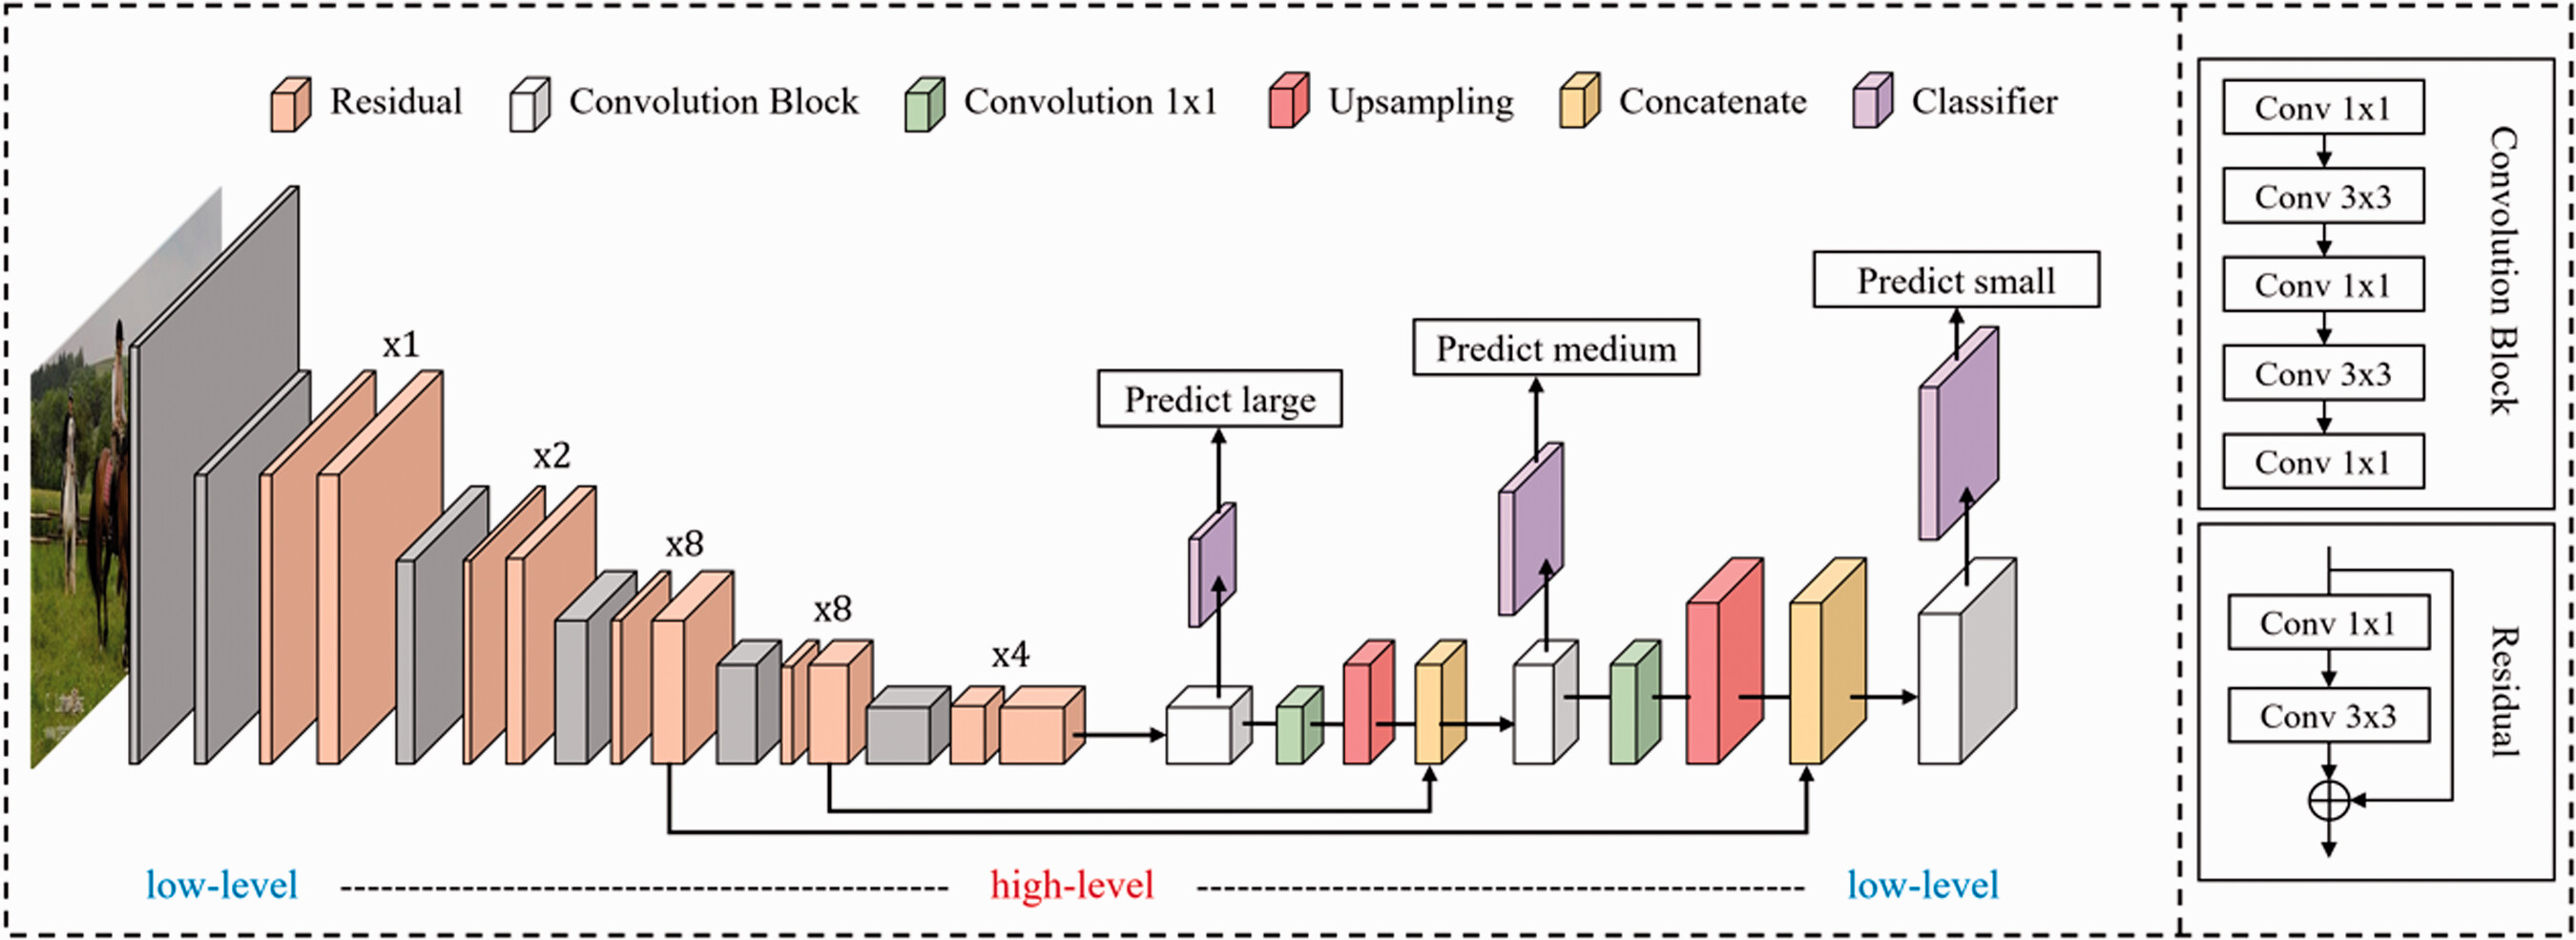
\includegraphics[width=16cm, height=5cm]{yolodos}
    \caption{Esquema de redes neuronales de YOLOv3.\protect\footnotemark}
    \label{fig:mesh1}
\end{figure}



\section{Objetivos y alcance}

\footnotetext{Imagen tomada de \url{https://journals.sagepub.com/cms/10.1177/0020720920983524/asset/images/large/10.1177_0020720920983524-fig2.jpeg}}

A continuación, se presentan los requisitos establecidos en la etapa de apertura del trabajo y su estado actual a la fecha. Es necesario tener en cuenta que, debido a cambios operativos, algunos de estos requisitos no pudieron ser cumplidos en su totalidad. \\ 

\begin{enumerate}
\item Requerimientos funcionales:
\begin{enumerate}
	\item El módulo debe detectar personas o animales de gran porte en áreas que el cliente defina como restringidas.
	\begin{itemize}
		\item Tipo: obligatorio
		\item Estado: finalizado
	\end{itemize}
	\item El módulo debe ser capaz de detectar a un intruso en un tiempo no mayor a 4 segundos.
	\begin{itemize}
		\item Tipo: obligatorio
		\item Estado: finalizado
	\end{itemize}
	\item El módulo debe correr en un computador de uso de hogar. Este debe ser comparable o menor a un Intel Core I5 y con no más de 8 GB de memoria RAM.
	\begin{itemize}
		\item Tipo: obligatorio
		\item Estado: finalizado
	\end{itemize}
	\item El sistema debe ser capaz de reconocer la presencia de intrusos, aun cuando el vídeo se haya registrado con el dron en movimiento.
	\begin{itemize}
		\item Tipo: obligatorio
		\item Estado: finalizado
	\end{itemize}
	\item \textbf{Requerimiento Opcional:} el sistema debe correr en un equipo que quepa a bordo de los drones (una Raspberry Pi, por ejemplo). 
	\begin{itemize}
		\item Tipo: opcional
		\item Estado: descartado
	\end{itemize}
\end{enumerate}
\item Requerimientos de documentación:
\begin{enumerate}
	\item El sistema deberá contar con un manual de usuario.
	\begin{itemize}
		\item Tipo: obligatorio
		\item Estado: finalizado
	\end{itemize}
	\item Se deberá contar con un manual de instalación del módulo desarrollado.
	\begin{itemize}
	 \item Tipo:obligatorio
	 \item Estado: finalizado
	\end{itemize}
	\item El código fuente deberá estar debidamente comentado.
	\begin{itemize}
		\item Tipo: obligatorio
		\item Estado : finalizado
	\end{itemize}
\end{enumerate}
\item Requerimientos de pruebas:
\begin{enumerate}
	\item El módulo deberá ser probado formalmente según indicaciones del cliente.
	\begin{itemize}
		\item Tipo: requisito modificado
		\item Estado: descartado
	\end{itemize}
	\item El cliente debe poder acceder en cualquier momento a la versión más reciente del código a través de GitHub.
	\begin{itemize}
	 \item Tipo: obligatorio
	 \item Estado: finalizado
	\end{itemize}
\end{enumerate}
\item Requerimientos de la interfaz:
\begin{enumerate}
	\item El usuario debe poder iniciar fácilmente la ejecución del módulo.
	\begin{itemize}
		\item Tipo: obligatorio
		\item Estado: finalizado
	\end{itemize}
\end{enumerate}
\item Requerimientos de interoperabilidad:
\begin{enumerate}
	\item \textbf{Opción A:} el módulo debe estar en capacidad de recibir el \textit{streaming} de vídeo de entre 4 y 8 drones.
	\begin{itemize}
		\item Tipo: requisito modificado
		\item Estado: descartado
	\end{itemize}
	\item \textbf{Opción B:} el módulo debe ser capaz de recibir un \textit{streaming} de vídeo y ejecutar la detección de intrusos en hardware dedicado a bordo.
	\begin{itemize}
		\item Tipo: requisito modificado
		\item Estado: descartado
	\end{itemize}
	\item Se requiere que el sistema pueda conectarse con otro módulo capaz de tomar decisiones con base en la información de detección de intrusos.
	\begin{itemize}
		\item Tipo: obligatorio
		\item Estado: finalizado
	\end{itemize}
\end{enumerate}
\end{enumerate}


A pesar de que algunos de los requerimientos funcionales fueron descartados dados algunos cambios que se presentaron en las plataformas del cliente, también hubo requerimientos que fueron agregados:

\begin{enumerate}
\setcounter{enumi}{5}
\item Requerimientos nuevos:
\begin{enumerate}
	\item El módulo deberá retransmitir los \textit{frames} procesados a un servidor indicado por el cliente. 
	\begin{itemize}
		\item Tipo: obligatorio
		\item Estado: finalizado
	\end{itemize}
\end{enumerate}
\end{enumerate}

Es importante tener en cuenta que el trabajo no contempló:

\begin{itemize}

	\item Reconocimiento del intruso: es decir, en caso de que se detecte a una persona, no se deberá dar con su identidad.
	
	\item Reacción del dron: es decir, una vez se haya detectado satisfactoriamente a un intruso, el sistema no deberá dar instrucciones específicas al dron, por ejemplo, de seguirlo.
	
	\item No existen requisitos específicos de cómo realizar la retransmisión de los \textit{frames} ya procesados.

\end{itemize}



